
\documentclass{article}
\title{Report 4: Threads}
\author{Nguyen Dang Minh - M23.ICT.008}
\date{\today}

\usepackage{booktabs}
\usepackage{amsmath}
\usepackage{listings} % For code listings
\usepackage{xcolor}   % For defining colors
\usepackage{graphicx} 
\usepackage{float}

% Define custom colors
\definecolor{codegray}{rgb}{0.95, 0.95, 0.95}
\definecolor{codepurple}{rgb}{0.58, 0, 0.82}

% Define lstlisting style
\lstdefinestyle{mystyle}{
    backgroundcolor=\color{codegray},   % Background color
    basicstyle=\footnotesize\ttfamily,  % Font style
    breaklines=true,                     % Automatically break lines
    captionpos=b,                        % Position of the caption
    commentstyle=\color{codepurple},     % Comment style
    keywordstyle=\color{blue},           % Keyword style
    language=Python,                     % Language for syntax highlighting
    numbers=left,                        % Line numbers on the left
    numbersep=5pt,                       % Space between line numbers and code
    showstringspaces=false,              % Don't show spaces in strings
    stringstyle=\color{codepurple},      % String literal style
    tabsize=4                            % Tab size
}

% Set default lstlisting style to mystyle
\lstset{style=mystyle}
\begin{document}

\maketitle
\section{Tasks:}

Apply grayscale to this image:

\begin{figure}[H]
    \centering
    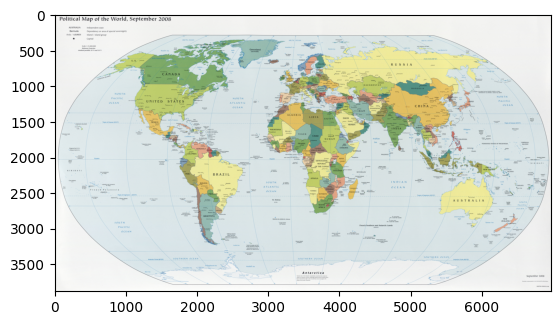
\includegraphics[width=1\linewidth]{output.png}
\end{figure} 
Information: 
\begin{itemize}
    \item Height: 3880
    \item Weight: 6972
    \item Channel: 3
\end{itemize}


\section{Running using CPU}


We defined a function to convert an image to grayscale on the CPU. 
\begin{lstlisting}[language=Python]
for i in range(H):
  for j in range(W):
    g = np.uint8((float(image[i][j][0]) + float(image[i][j][1]) + float(image[i][j][2])) // 3)
    array[i][j]= [g]*3
    del g
\end{lstlisting}
It isn't scale good at all.

\begin{figure}[H]
    \centering
    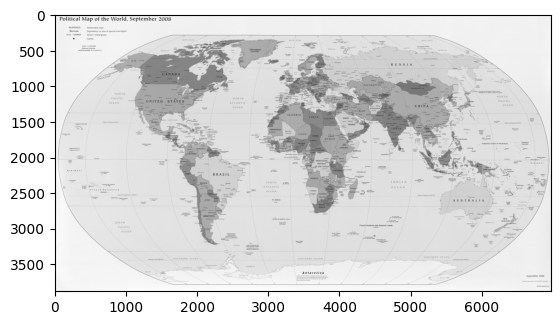
\includegraphics[width=1\linewidth]{output2.png}
    \caption{Output}
    \label{fig:enter-label}
\end{figure}


Time elapsed :   83.45929431915283

\section{Running using GPU}

We defined a function to convert an image to grayscale on GPU.
\begin{lstlisting}[language=Python]
@cuda.jit
def grayscale(src, dst):
    tidx = cuda.threadIdx.x + cuda.blockIdx.x * cuda.blockDim.x
    g = np.uint8((src[tidx, 0] + src[tidx, 1] + src[tidx, 2]) / 3)
    dst[tidx, 0] = dst[tidx, 1] = dst[tidx, 2] = g
\end{lstlisting}

Time elapsed :  0.14880847930908203

x560 speed with GPU

\begin{figure}[H]
    \centering
    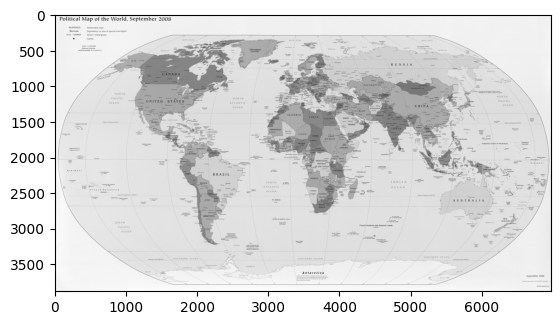
\includegraphics[width=1\linewidth]{output2.png}
    \caption{Output}
    \label{fig:enter-label}
\end{figure}


\section{Plot a graph of block size vs time}

We plot the time comparison between different block sizes. 
\begin{figure}[H]
    \centering
    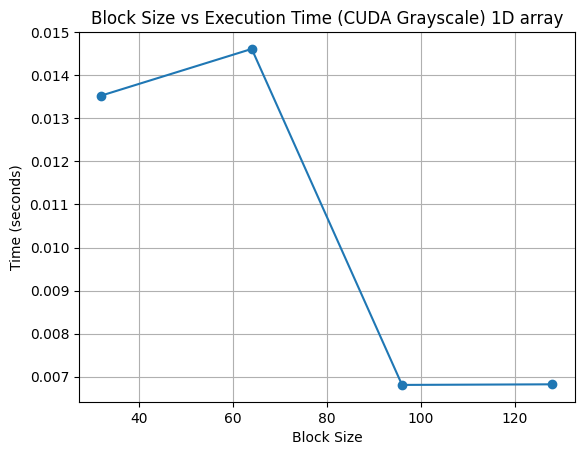
\includegraphics[width=0.76\linewidth]{output3.png}
\end{figure}

\begin{itemize}
    \item Block size = 32, Time = 0.013530492782592773
    \item Block size = 64, Time = 0.01461338996887207
    \item Block size = 96, Time = 0.0068094730377197266
    \item Block size = 128, Time = 0.006823539733886719
\end{itemize}


\begin{figure}[H]
    \centering
    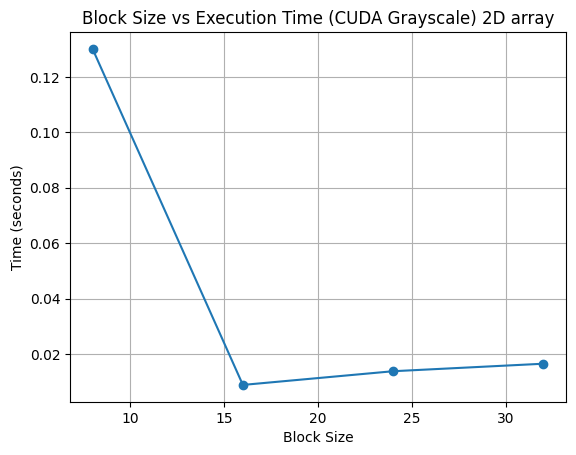
\includegraphics[width=0.76\linewidth]{output4.png}
\end{figure}

\begin{itemize}
    \item Block size = 8, Time = 0.13007044792175293
    \item Block size = 16, Time = 0.00886082649230957
    \item Block size = 24, Time = 0.013803958892822266
    \item Block size = 32, Time = 0.01651167869567871
\end{itemize}

\section{Conclusions}
\begin{itemize}
    \item GPU runtime is quite random and chaotics
    \item More block size seem better, but maybe to a limit.
\end{itemize}


\begin{itemize}
    \item 
\end{itemize}


\end{document}